\documentclass[11pt]{article}

% Change "review" to "final" to generate the final (sometimes called camera-ready) version.
% Change to "preprint" to generate a non-anonymous version with page numbers.
\usepackage[review]{acl}
% Standard package includes
\usepackage{times}
\usepackage{latexsym}

% For proper rendering and hyphenation of words containing Latin characters (including in bib files)
\usepackage[T1]{fontenc}
% For Vietnamese characters
% \usepackage[T5]{fontenc}
% See https://www.latex-project.org/help/documentation/encguide.pdf for other character sets

% This assumes your files are encoded as UTF8
\usepackage[utf8]{inputenc}

% This is not strictly necessary, and may be commented out,
% but it will improve the layout of the manuscript,
% and will typically save some space.
\usepackage{microtype}

% This is also not strictly necessary, and may be commented out.
% However, it will improve the aesthetics of text in
% the typewriter font.
\usepackage{inconsolata}
\usepackage{CJKutf8}
%Including images in your LaTeX document requires adding
%additional package(s)
\usepackage{graphicx}
\usepackage{booktabs}
\usepackage{float}
\usepackage{amssymb}
% If the title and author information does not fit in the area allocated, uncomment the following
%
%\setlength\titlebox{<dim>}
%
% and set <dim> to something 5cm or larger.

\title{When Translation Breaks Retrieval: Irreversible Error Propagation in Cross-lingual Medical Retrieval-Augmented Generation}

% Author information can be set in various styles:
% For several authors from the same institution:
% \author{Author 1 \and ... \and Author n \\
%         Address line \\ ... \\ Address line}
% if the names do not fit well on one line use
%         Author 1 \\ {\bf Author 2} \\ ... \\ {\bf Author n} \\
% For authors from different institutions:
% \author{Author 1 \\ Address line \\  ... \\ Address line
%         \And  ... \And
%         Author n \\ Address line \\ ... \\ Address line}
% To start a separate ``row'' of authors use \AND, as in
% \author{Author 1 \\ Address line \\  ... \\ Address line
%         \AND
%         Author 2 \\ Address line \\ ... \\ Address line \And
%         Author 3 \\ Address line \\ ... \\ Address line}

\author{First Author \\
  Affiliation / Address line 1 \\
  Affiliation / Address line 2 \\
  Affiliation / Address line 3 \\
  \texttt{email@domain} \\\And
  Second Author \\
  Affiliation / Address line 1 \\
  Affiliation / Address line 2 \\
  Affiliation / Address line 3 \\
  \texttt{email@domain} \\}

%\author{
%  \textbf{First Author\textsuperscript{1}},
%  \textbf{Second Author\textsuperscript{1,2}},
%  \textbf{Third T. Author\textsuperscript{1}},
%  \textbf{Fourth Author\textsuperscript{1}},
%\\
%  \textbf{Fifth Author\textsuperscript{1,2}},
%  \textbf{Sixth Author\textsuperscript{1}},
%  \textbf{Seventh Author\textsuperscript{1}},
%  \textbf{Eighth Author \textsuperscript{1,2,3,4}},
%\\
%  \textbf{Ninth Author\textsuperscript{1}},
%  \textbf{Tenth Author\textsuperscript{1}},
%  \textbf{Eleventh E. Author\textsuperscript{1,2,3,4,5}},
%  \textbf{Twelfth Author\textsuperscript{1}},
%\\
%  \textbf{Thirteenth Author\textsuperscript{3}},
%  \textbf{Fourteenth F. Author\textsuperscript{2,4}},
%  \textbf{Fifteenth Author\textsuperscript{1}},
%  \textbf{Sixteenth Author\textsuperscript{1}},
%\\
%  \textbf{Seventeenth S. Author\textsuperscript{4,5}},
%  \textbf{Eighteenth Author\textsuperscript{3,4}},
%  \textbf{Nineteenth N. Author\textsuperscript{2,5}},
%  \textbf{Twentieth Author\textsuperscript{1}}
%\\
%\\
%  \textsuperscript{1}Affiliation 1,
%  \textsuperscript{2}Affiliation 2,
%  \textsuperscript{3}Affiliation 3,
%  \textsuperscript{4}Affiliation 4,
%  \textsuperscript{5}Affiliation 5
%\\
%  \small{
%    \textbf{Correspondence:} \href{mailto:email@domain}{email@domain}
%  }
%}
\setlength{\textfloatsep}{10pt plus 2pt minus 2pt}
\setlength{\intextsep}{10pt plus 2pt minus 2pt}
\setlength{\floatsep}{10pt plus 2pt minus 2pt}
\begin{document}
\begin{CJK}{UTF8}{gbsn}
\maketitle
\begin{abstract}
Cross-lingual medical retrieval-augmented generation (RAG) often translates non-English clinical queries into English before retrieval. We find that, in this pipeline, translation errors introduced at this step can substantially alter retrieval, and post-hoc query correction does not recover performance unless retrieval is repeated. Retrieval adds little when translation is faithful (54.0\% without retrieval vs.\ 55.5\% with it), but can become harmful once translation is corrupted, costing 20 points relative to no retrieval at all. We study this mechanism using 200 Chinese medical multiple-choice questions from CMB-Exam and an English biomedical retrieval corpus derived from PubMedQA. Helsinki-NLP machine translation causes a 21.5-percentage-point accuracy drop relative to high-quality translation; in a controlled experiment, correcting the query without re-retrieval does not recover this gap and can actively lower performance. Retrieval-level analysis reveals that machine-translated queries retrieve entirely disjoint document sets in 65.5\% of cases (mean Jaccard $= 0.125$). Of the 200 questions, 50 (25.0\%) succeed under high-quality translation but fail under machine translation; 82 (41.0\%) fail under both, pointing to corpus coverage gaps and limitations in retrieval or generation rather than translation quality. In this pipeline, translation is therefore not a modular preprocessing step that can be corrected after the fact: once retrieval has occurred, the errors it introduced cannot be undone.
\end{abstract}

\section{Introduction}
\label{sec:intro}
Medical question answering systems increasingly rely on retrieval-augmented generation (RAG) \cite{NEURIPS2020_6b493230}, which grounds model responses in external evidence retrieved via dense passage retrieval \cite{karpukhin2020dense}, reducing hallucination and improving factual accuracy in knowledge-intensive tasks. In monolingual settings, the pipeline assumption is simple: the query used for retrieval accurately reflects the user’s clinical information requirements. However, in multilingual settings, this assumption is influenced by the translation process. A Chinese medical question cannot be matched directly against an English biomedical corpus constructed from resources such as PubMedQA \cite{jin-etal-2019-pubmedqa}. It must first be translated into English, embedded, and then searched. This translation step sits at the entrance to the pipeline. If it distorts a drug name, inverts a clinical relationship, or replaces a symptom description with a semantically unrelated phrase, the retrieval index will receive a query that no longer represents the original clinical question. The resulting documents may be irrelevant, incomplete, or misleading --- and the generator will answer from that compromised evidence set.
  
Prior work on medical question answering has focused on model capability: benchmark performance, clinical reasoning, and domain-adapted models \cite{thirunavukarasu2023large, achiam2023gpt, tsatsaronis2012bioasq}. Few prior studies have asked the more fundamental question: once a translation error has distorted the query and shaped retrieval, can the pipeline recover?
  
In this paper, we study whether translation errors in this cross-lingual medical RAG pipeline can be recovered after retrieval has already occurred: once a mistranslated query has shaped the retrieved document set, downstream correction alone cannot recover the evidence that was never retrieved. This mechanism matters not because retrieval contributes much on average---it adds little when the query is faithful (55.5\% vs. 54.0\% without retrieval)---but because its failure mode is asymmetric: corrupted retrieval costs 20 points relative to no retrieval at all, and this cost is unreachable by any correction applied after the retrieval step. We study this mechanism using 200 Chinese single-answer multiple-choice questions from CMB-Exam \cite{wang-etal-2024-cmb} and an English biomedical retrieval corpus derived from PubMedQA \cite{jin-etal-2019-pubmedqa}. We compare a high-quality translation condition against Helsinki-NLP machine translation \cite{tiedemann-thottingal-2020-opus}, and evaluate a set of post-translation correction interventions as diagnostic probes rather than competing translation systems. We also examine whether the translation quality of answer options independently predicts pipeline failure, separating this effect from query-level mistranslation. Our goal is to measure how much of the performance gap caused by poor translation can be recovered once the translated query has entered the retrieval pipeline.

This paper is organized around four research questions:
\begin{enumerate}
\item[\textbf{RQ1}:] How much does machine translation of Chinese medical queries degrade end-to-end answer accuracy compared to high-quality translation?
\item[\textbf{RQ2}:] Which translation error types (terminology error, syntactic distortion, and semantic drift) contribute most to downstream answer failure? 
\item[\textbf{RQ3}:] Can post-translation correction interventions recover the performance gap, and is this recovery attributable to query improvement or to re-retrieval?
\item[\textbf{RQ4}:] Does answer-option translation quality independently predict RAG failure, or is query mistranslation the primary driver?
\end{enumerate}


To address these questions, we make four main contributions:
\begin{itemize}
\item We quantify the performance degradation caused by machine translation in a cross-lingual medical RAG pipeline, showing a 21.5-percentage-point drop in answer accuracy from high-quality to raw machine translation; 25.0\% of questions (C1 correct, C2 incorrect) show failures directly attributable to translation degradation, and 41.0\% fail under both C1 and C2, a joint failure rate we attribute to a combination of corpus coverage gaps, retrieval limitations, and generation limitations, rather than to translation quality alone.

\item We analyze three translation error types (terminology error, syntactic distortion, and semantic drift) and show that they co-occur rather than acting as separable failure modes: all three appear together in 53 of 200 questions, only 4 show none, and these all-three questions have the lowest accuracy (25\%), indicating that co-occurrence rather than any single type drives failure (\S\ref{sec:error_impact}). We further show that answer-option mistranslation independently reduces accuracy by 16.5 percentage points, even when query retrieval is unaffected.

\item We show that, in this pipeline, correction interventions recover performance only when re-retrieval is permitted, not when applied post-hoc to a fixed retrieved document set (\S\ref{sec:irreversibility}). Machine-translated queries diverge from high-quality queries in 65.5\% of cases (mean Jaccard $= 0.125$), providing direct retrieval-level evidence for translation-induced pipeline failure.

\item We show that a multilingual embedding baseline matches high-quality translation (58.0\% vs.\ 55.5\%, $p = 0.522$), so our diagnostic study targets settings where switching to a translation-free paradigm may not be immediately feasible (e.g., fixed monolingual infrastructure, audit-trail requirements).
\end{itemize}

\section{Related Work}
\subsection{Retrieval-Augmented Generation}
Retrieval-augmented generation combines a retrieval component with a generative model to ground responses in external evidence \cite{NEURIPS2020_6b493230}. Dense retrieval methods using learned embeddings \cite{karpukhin2020dense, reimers-gurevych-2019-sentence} have shown superior performance over traditional sparse retrieval methods such as BM25 in many open-domain question answering tasks. Domain adaptation of RAG pipelines has been shown to improve performance in specialized settings \cite{siriwardhana2023improving}. Evaluation across diverse retrieval tasks has revealed substantial variation in zero-shot generalization \cite{thakur2021beir}. Our work extends this line of research to the multilingual medical setting, where the translation step introduces an additional source of error before retrieval.

\subsection{Medical Question Answering}
Medical question answering has been studied using a range of biomedical benchmarks \cite{jin-etal-2019-pubmedqa, tsatsaronis2012bioasq}. Large language models have demonstrated strong performance on medical examinations and clinical tasks \cite{thirunavukarasu2023large, achiam2023gpt}. Chinese medical benchmarks provide evaluation resources in non-English clinical contexts \cite{wang-etal-2024-cmb}. However, most existing work evaluates models in monolingual settings and does not examine how translation affects retrieval-based pipelines.

\subsection{Multilingual and Cross-lingual Retrieval}
Cross-lingual retrieval work \cite{nie2010cross,longpre2021mkqa,asai2021xor,zhang-etal-2021-mr,nie2023cross} has studied cross-lingual alignment at the retrieval model level. We study instead how query mistranslation propagates error through a fixed retrieval pipeline, treating translation quality as the primary variable.

\subsection{Translation Quality and Hallucination Detection}
Translation artifacts systematically distort downstream NLP tasks \cite{artetxe2020translation, guerreiro2023hallucinations}, and OPUS-MT provides accessible but domain-limited translation \cite{tiedemann-thottingal-2020-opus}. Reference-free MT quality estimation \cite{rei2020comet, ranasinghe2020transquest} operates at the translation level; our BERTScore-based signal, following SelfCheckGPT \cite{manakul-etal-2023-selfcheckgpt}, operates at the pipeline output level. We develop a three-category error taxonomy specific to cross-lingual medical RAG.


\section{Methodology}
\subsection{Dataset and Retrieval Corpus}
We use 200 single-answer multiple-choice questions randomly sampled (seed=42) from a pool of 10,035 CMB-Exam questions \cite{wang-etal-2024-cmb}, covering clinical medicine, pharmacology, and basic science. Each question presents five Chinese-language options with one correct answer.  The retrieval corpus consists of 852,618 unique PubMed abstracts associated with the PubMedQA source corpus \cite{jin-etal-2019-pubmedqa}. The corpus is encoded using all-MiniLM-L6-v2 \cite{reimers-gurevych-2019-sentence} and indexed with FAISS IndexFlatL2 \cite{johnson2019billion}. At inference time, the top $k=3$ abstracts are retrieved for each translated query and concatenated as context. Answer generation is performed by GPT-4o-mini\footnote{OpenAI, \url{https://platform.openai.com} (gpt-4o-mini), accessed May 2026.}, which receives the retrieved context and translated question with options in a fixed prompt template.

\subsection{Translation and Experimental Conditions}
We design a set of controlled conditions to isolate the contribution of translation quality to pipeline performance. These are diagnostic probes, not competing translation systems; the retrieval and generation components are held constant across all conditions. C1 uses GPT-4o-mini translation as the high-quality condition: not a gold standard, but a reproducible practical ceiling. To check that C1 does not underestimate that ceiling, we additionally run C1' using GPT-4.1\footnote{OpenAI, \url{https://platform.openai.com} (\texttt{gpt-4.1-2025-04-14}), accessed May 2026.} (\S\ref{sec:controls}). To assess whether the translate-then-retrieve paradigm is necessary, we additionally run a translation-free baseline (C0) using a multilingual embedding model (\texttt{paraphrase-multilingual-MiniLM-L12-v2}; hereafter \texttt{mMiniLM})\footnote{Sentence-Transformers, \url{https://huggingface.co/sentence-transformers/paraphrase-multilingual-MiniLM-L12-v2}, accessed June 2026.} that encodes Chinese queries directly without translation (\S\ref{sec:controls}). C2 (Helsinki-NLP \cite{tiedemann-thottingal-2020-opus} machine translation, no correction) establishes the MT baseline floor. Four conditions apply post-hoc correction to C2 output: C3 (GPT-4o-mini, general correction), C3b (GPT-4o-mini, restricted to terminology replacement; an ablation of C3), C4 (DeepSeek V4-Flash\footnote{DeepSeek, \url{https://api.deepseek.com} (deepseek-v4-flash), accessed May 2026.}, a different model family), and C5 (GPT-5.5\footnote{OpenAI, \url{https://platform.openai.com} (gpt-5.5), accessed May 2026.}, a stronger model). Together they probe correction strategy (C3 vs.\ C3b) and the ceiling of correction capability across families and scales (C4, C5).

We additionally include two control conditions: (1) Claude Sonnet 4.6\footnote{Anthropic, \url{https://www.anthropic.com} (claude-sonnet-4-6), accessed June 2026.} generation on C1 translations, to control for model self-consistency, and (2) a post-hoc retrieval-fixed condition (C2a) in which corrected queries from C3 or C5 are paired with
C2-retrieved documents, to isolate the contribution of re-retrieval from query correction. To isolate the independent contribution of option translation quality, we construct two option-substitution ablations: \textbf{C1q+C2o} pairs C1 queries and retrieved documents with C2 option translations, and \textbf{C2q+C1o} pairs C2 queries and retrieved documents with C1 option translations.

\subsection{Error Taxonomy}
\label{sec:taxonomy}
We develop a three-category taxonomy to characterize errors in C2 translations, derived from inspection of recurring error patterns in C2 outputs. \textbf{T1 (terminology error)}: medical terms are mistranslated or rendered nonsensically. \textbf{T2 (syntactic distortion)}: sentence structure is corrupted at the grammatical level, such as clause reordering, dropped negations, or broken subject-verb relationships, making the sentence uninterpretable or structurally incoherent. \textbf{T3 (semantic drift)}: the translated sentence is grammatically well-formed but conveys a meaning that diverges significantly from the source, without a single identifiable terminology error. These categories are non-exclusive; a single translation may exhibit multiple error types simultaneously.

GPT-4o-mini automatically labeled all 200 C2 translations according to this taxonomy. Three annotators validated a 60-question sample; one was excluded as an outlier (details in Limitations). Across the two retained annotators, human--GPT Jaccard was 0.636 (mean) and inter-annotator Jaccard was 0.492, moderate for a non-exclusive multi-label task. The two diverged systematically on the T2/T3 boundary, indicating that syntactic distortion and semantic drift are not cleanly separable under our definitions. We note a potential circularity: GPT-4o-mini both annotates errors and serves as the C3 corrector, and may miss the hard errors it fails to correct. To bound this effect, we checked whether the two failures coincide within the 60-question validation sample. Taking either retained annotator's labels as the reference, GPT-4o-mini missed at least one human-labeled error type on 36 items and C3 answered 35 incorrectly; the two coincide on 21, against 21.0 expected under independence. Annotation misses are therefore not concentrated on the items correction fails to fix. Answer-option translation quality is assessed automatically using GPT-4o-mini at temperature=0. For each question, each of the five options is scored on a three-point scale: 1 (Good: meaning preserved, terminology correct), 2 (Partial: meaning partially preserved, some errors), or 3 (Bad: meaning lost or completely wrong). The average score across all five options is used as a continuous quality indicator for correlation analysis.

\subsection{Evaluation Metrics}
For each condition, the translated question, its options, and the top $k=3$ retrieved PubMed abstracts are given to GPT-4o-mini, which is prompted to reply with a single option letter (A--E) at temperature=0. To reduce stochasticity arising from non-deterministic API sampling, this process is repeated three times and the majority vote is taken as the final answer. Accuracy is computed by comparing the selected option against the ground-truth label.

Pairwise comparisons between conditions are evaluated using McNemar's test on the binary correct/incorrect outcomes for each question, with a significance threshold of $p < 0.05$.

We treat C1-vs-C2 and C2-vs-correction comparisons as pre-specified primary tests; within-correction comparisons (C3 vs.\ C4, C3 vs.\ C5, C4 vs.\ C5, C3 vs.\ C3b) are exploratory and interpreted without multiplicity correction. Under Bonferroni correction for 11 pairwise tests ($\alpha = 0.0045$), the C2 vs.\ C5 result ($p = 0.003$) falls at the boundary; the C4 vs.\ C5 result ($p = 0.018$) does not survive correction.

To assess output consistency as a reliability proxy, we apply SelfCheckGPT \cite{manakul-etal-2023-selfcheckgpt} with BERTScore (\texttt{microsoft/deberta-xlarge-mnli}). For each question, three independent samples are generated at temperature=1.0; lower inter-sample consistency indicates higher hallucination risk.

\section{Results}
\label{sec:results}
\subsection{Main Accuracy Results}
Figure~\ref{fig:accuracy} shows accuracy across all six conditions. High-quality translation GPT-4o-mini (C1) achieves 55.5\%, while raw machine translation from Helsinki-NLP (C2) drops to 34.0\%, a 21.5-percentage-point decline. Of the 200 questions, 50 (25.0\%) are translation-sensitive (C1 correct, C2 incorrect), representing failures more directly attributable to translation degradation; 82 (41.0\%) fail under both conditions --- a joint failure rate we attribute to a combination of corpus coverage gaps, retrieval-model limitations, and generation failures rather than to translation quality alone (see \S\ref{sec:retrieval_impact}). Post-translation correction recovers part of this gap: C3 reaches 38.5\%, C3b reaches 39.0\%, C4 reaches 36.0\%, and C5 reaches 43.5\%. Even the strongest correction intervention leaves a 12-point gap below C1.

\begin{figure}[t]
\centering
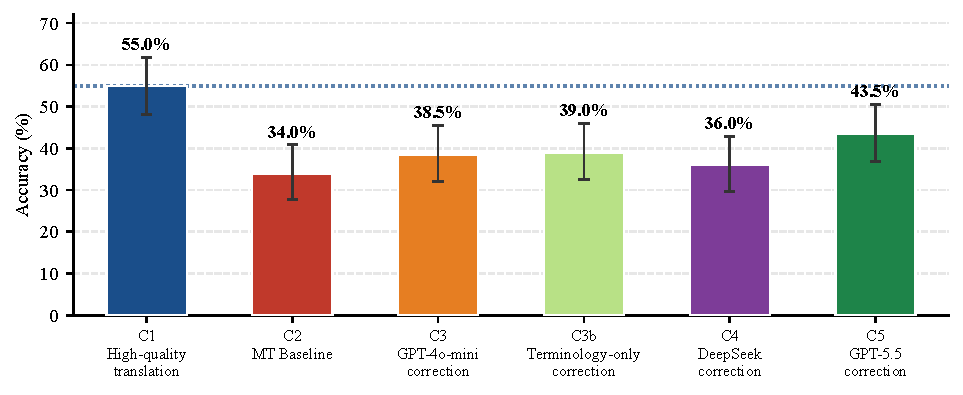
\includegraphics[width=\columnwidth]{fig1_accuracy.pdf}
\caption{Accuracy across experimental conditions.
The dotted line marks the C1 high-quality translation condition (55.5\%).}
\label{fig:accuracy}
\end{figure}

McNemar's test confirms that C1 significantly outperforms all other conditions (all $p < 0.01$). Among correction conditions, only C5 achieves a statistically significant improvement over raw machine translation ($p = 0.003$), though this result sits at the Bonferroni-corrected boundary ($\alpha = 0.0045$) and should be interpreted with caution. C3 and C4 do not differ significantly from C2 ($p = 0.151$ and $p = 0.343$ respectively). C3 and C3b are statistically identical ($p = 1.000$), indicating that restricting correction to terminology does not alter model behavior. Table~\ref{tab:significance} reports all pairwise comparisons.


\begin{table}[ht]
\centering
\begin{tabular}{llr}
\toprule
\textbf{Comparison} & \textbf{$p$-value} & \textbf{Significant} \\
\midrule
C1 vs.\ C2 & $<$0.0001 & Yes \\
C1 vs.\ C3 & $<$0.0001 & Yes \\
C1 vs.\ C4 & $<$0.0001 & Yes \\
C1 vs.\ C5 & 0.004 & Yes \\
C2 vs.\ C3 & 0.151 & No \\
C2 vs.\ C4 & 0.343 & No \\
C2 vs.\ C5 & 0.003 & Yes \\
C3 vs.\ C4 & 0.458 & No \\
C3 vs.\ C5 & 0.144 & No \\
C4 vs.\ C5 & 0.018 & Yes$^*$ \\
C3 vs.\ C3b & 1.000 & No \\
\bottomrule
\end{tabular}
\caption{Pairwise McNemar's test results. $^*$Significant at $p < 0.05$ but does not survive Bonferroni correction ($\alpha = 0.0045$ for 11 comparisons).}
\label{tab:significance}
\end{table}

\subsection{No-Retrieval Baseline}
\label{sec:norag}
To assess how much of C1's accuracy is attributable to retrieval rather than the generator's own parametric medical knowledge, we ran GPT-4o-mini on the same C1-translated questions and options with no retrieved context at all, using an otherwise identical protocol (three runs at temperature=0, single-letter output, majority vote). This no-retrieval baseline reaches 54.0\%, statistically indistinguishable from C1 (55.5\%; McNemar's $p = 0.755$; Bonferroni-corrected $\alpha = 0.025$ for this two-comparison family). On this benchmark, retrieval adds only modest marginal benefit over the generator’s parametric knowledge when translation is high-quality: GPT-4o-mini already answers a majority of these questions from its own training knowledge.

The comparison against C2 is more informative. The no-retrieval baseline (54.0\%) significantly outperforms C2 (34.0\%; McNemar's $p < 0.0001$), with 51 questions answered correctly without any context but incorrectly under C2, against only 11 in the opposite direction. On this benchmark, corrupted retrieval performs substantially worse than no retrieval, suggesting that irrelevant retrieved context can be worse than no context at all.

\subsection{Control Conditions}
\label{sec:controls}
Two further controls bound the interpretation of C1. C1' (GPT-4.1
translation) reaches 56.5\%, indistinguishable from C1 ($p = 0.851$),
so C1 does not materially underestimate the practical translation
ceiling. C0 (\texttt{mMiniLM}, no translation) reaches 58.0\%, also
comparable to C1 ($p = 0.522$).

Taken with the no-retrieval baseline (\S\ref{sec:norag}), C1, C1', C0,
and no-retrieval all fall within a narrow 54.0--58.0\% band that is
insensitive to the translation model, to the translation step itself,
and to the presence of retrieval. The 21.5-point drop to C2 is therefore consistent with a threshold effect: degradation appears once translation quality falls far enough to divert retrieval. The Claude Sonnet 4.6 self-consistency control is discussed in \S\ref{sec:discussion}.

\subsection{Translation Error Classification}
Table~\ref{tab:error_types} reports the frequency of three translation error types across the 200 machine-translated questions. Terminology errors (T1) are present in 95.5\% of questions. Semantic drift (T3) affects 84.0\%. Syntactic distortion (T2) appears in 38.5\%. Only 4 questions (2.0\%) contain no translation errors. Multiple error types often occur simultaneously: all three were present in 53 questions. Appendix~\ref{sec:appendix_cases} presents five representative cases.

\begin{table}[ht]
\centering
\begin{tabular}{lrr}
\toprule
\textbf{Error Type} & \textbf{Count} & \textbf{Proportion} \\
\midrule
T1: Terminology error & 191 & 95.5\% \\
T2: Syntactic distortion & 77 & 38.5\% \\
T3: Semantic drift & 168 & 84.0\% \\
No error & 4 & 2.0\% \\
\bottomrule
\end{tabular}
\caption{Translation error frequency in C2 (n=200). Error types are not mutually exclusive.}
\label{tab:error_types}
\end{table}

\subsection{Impact of Error Types on Accuracy}
\label{sec:error_impact}
The T1-only subgroup ($n=5$) is omitted from the figure due to insufficient sample size for reliable estimation.  Figure~\ref{fig:error_types} shows accuracy across four error-type subgroups for conditions C2, C3, and C5. Individual error-type subgroups do not separate cleanly: T1 and T3 produce similar C2 accuracy (34\% and 33\% respectively), and the T2 subgroup's lower accuracy (26\%) is difficult to attribute to syntactic distortion specifically, since 53 of the 77 T2 items (68.8\%) also carry both T1 and T3 (\S\ref{sec:taxonomy}). The clearer pattern is at the level of combination: questions with all three error types drop to 25\% accuracy, the lowest among all subgroups, consistent with error co-occurrence rather than any single error type driving failure. The C3/C5 reversal in the all-three subgroup (34.0\% vs.\ 32.0\%) is not significant ($p = 1.000$, $n = 53$; discordant pairs 5 vs.\ 4), reflecting sampling variance. We note that the T2/T3 boundary showed low inter-annotator agreement (\S\ref{sec:taxonomy}); subgroup results for these two categories should therefore be read as indicative rather than as clean separations.

\begin{figure}[t]
\centering
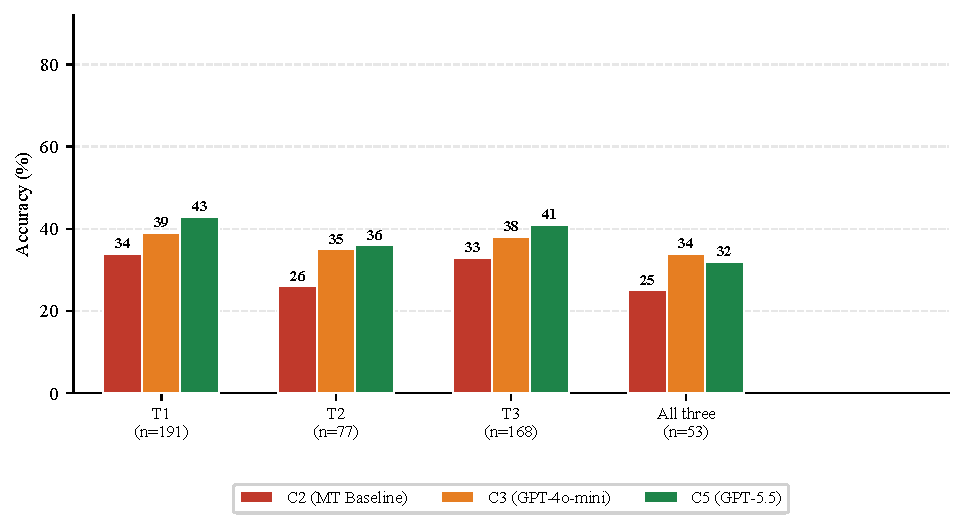
\includegraphics[width=\columnwidth]{fig2_error_types.pdf}
\caption{Accuracy by translation error type across conditions C2, C3, and C5.}
\label{fig:error_types}
\end{figure}

\subsection{Answer-Option Translation Quality}
\label{sec:option_quality}
Table~\ref{tab:option_quality} reports accuracy stratified by answer-option translation quality. The Pearson correlation between option quality score and accuracy is $r = -0.068$ ($p = 0.340$), which is not statistically significant. Option translation quality does not predict answer accuracy independently of query translation quality.

\begin{table}[ht]
\centering
\begin{tabular}{lrrrr}
\toprule
\textbf{Option Quality} & \textbf{n} & \textbf{C2} & \textbf{C3} & \textbf{C5} \\
\midrule
Good & 47 & 38\% & 32\% & 47\% \\
Partial & 104 & 35\% & 40\% & 41\% \\
Bad & 49 & 29\% & 41\% & 45\% \\
\bottomrule
\end{tabular}
\caption{Accuracy by answer-option translation quality. Correlation with accuracy: $r = -0.068$, $p = 0.340$. Option quality scores are GPT-4o-mini automated assessments (1=Good, 2=Partial, 3=Bad), averaged across five options per question.}
\label{tab:option_quality}
\end{table}


\subsection{Query versus Option Mistranslation}
We directly manipulate option quality by substitution: \textbf{C1q+C2o} pairs C1 queries and documents with C2 options, and \textbf{C2q+C1o} pairs C2 queries and documents with C1 options.

C1q+C2o achieves 39.0\%, a significant 16.5-point drop from C1 ($p < 0.0001$): option mistranslation independently causes substantial loss even when retrieval is unaffected. C2q+C1o achieves 31.5\%, not significantly different from C2 ($p = 0.533$). Query mistranslation is therefore the primary bottleneck: correcting options cannot compensate for retrieval damage already done.

\subsection{SelfCheckGPT Consistency}
\label{sec:selfcheck}
BERTScore inconsistency correlates with question-level accuracy ($r = -0.185$, $p = 0.009$, $n = 200$), a weak but statistically significant signal suggesting that output stability tracks translation-induced reliability risk. A condition-level association is also present but is based on only six conditions ($n=6$); with so few points, a Pearson correlation and its associated $p$-value are not a meaningful measure of strength, so we report it descriptively in Appendix~\ref{sec:appendix_selfcheck} rather than in the main text.

\subsection{Retrieval-Level Impact of Translation Quality}
\label{sec:retrieval_impact}
To assess whether translation errors cause retrieval divergence independently of answer accuracy, we computed the Jaccard similarity between the top-$k$ documents retrieved under C1 and C2 for each of the 200 questions. The mean Jaccard similarity is 0.125, indicating near-complete retrieval divergence between high-quality and machine-translated queries. In 65.5\% of questions, C1 and C2 retrieve entirely disjoint document sets (0/3 overlap); only 2.0\% of questions yield identical retrieval results (Table~\ref{tab:retrieval_overlap}). 

\begin{table}[ht]
\centering
\begin{tabular}{lrr}
\toprule
\textbf{Overlap (C1$\cap$C2)} & \textbf{$n$} & \textbf{C2 Accuracy} \\
\midrule
0/3 (disjoint) & 131 & 29.8\% \\
1/3 & 38 & 44.7\% \\
2/3 & 27 & 33.3\% \\
3/3 (identical) & 4 & 75.0\% \\
\bottomrule
\end{tabular}
\caption{C2 accuracy stratified by retrieval overlap with C1. Mean Jaccard similarity = 0.125.}
\label{tab:retrieval_overlap}
\end{table}

When C2 retrieves documents identical to C1 (overlap = 3/3), C2 accuracy rises to 75.0\%, though this subgroup is very small ($n = 4$). When retrieval is entirely disjoint (overlap = 0/3, 65.5\% of questions), C2 accuracy falls to 29.8\%. This overall association between retrieval overlap and answer accuracy is consistent with translation errors affecting the pipeline largely by diverting retrieval, whose downstream consequences are then realized at the generation stage (\S\ref{sec:irreversibility}). This retrieval divergence is robust to retrieval depth: mean Jaccard similarity remains low at $k=5$ (0.153) and $k=10$ (0.154), confirming that the finding is not an artifact of the choice $k=3$. Decomposing outcomes at the item level, 82 questions (41.0\%) fail under both C1 and C2 --- a floor attributable to corpus coverage gaps, retrieval limitations, generation failures, and residual C1 translation errors together --- while 50 (25.0\%) are correct under C1 but not C2. A further 7 questions are correct under C2 but not under C1, so high-quality translation does not strictly dominate machine translation item by item. The C1--C2 gap, therefore, reflects translation-sensitive failures that the joint-failure floor does not explain.


\subsection{Retrieval Irreversibility}
\label{sec:irreversibility}
To test whether retrieval damage can be recovered without repeating retrieval, we fix the top-$k$ documents retrieved under C2 and replace the query with the corrected translation from C3 or C5, preventing re-retrieval (condition C2a). This isolates query correction from retrieval re-execution.

Table~\ref{tab:c2a} reports the results. C2a\_C3 (C3-corrected query, C2-retrieved documents) achieves 26.0\%, below both C3 (38.5\%) and the C2 baseline (34.0\%). C2a\_C5 achieves 34.0\%, identical to C2 and 9.5 percentage points below C5 (43.5\%). Both C2a\_C3 vs.\ C3 and C2a\_C5 vs.\ C5 are statistically significant (McNemar's test, $p < 0.0001$). These results indicate that query correction applied after retrieval does not recover the lost performance in this setup and can reduce performance: improvement attributable to correction appears to depend on re-retrieval, not on improved query understanding at the generation stage.

\begin{table}[ht]
\centering
\begin{tabular}{p{3.8cm}cc}
\toprule
\textbf{Condition} & \textbf{Acc.} & \textbf{$p$} \\
\midrule
C2 (MT baseline) & 34.0\% & --- \\
C2a\_C3 (C3 query + C2 docs) & 26.0\% & --- \\
C3 (C3 query + C3 docs) & 38.5\% & $<$0.0001 \\
\midrule
C2a\_C5 (C5 query + C2 docs) & 34.0\% & --- \\
C5 (C5 query + C5 docs) & 43.5\% & $<$0.0001 \\
\bottomrule
\end{tabular}
\caption{Retrieval irreversibility experiment. C2a conditions fix C2-retrieved documents while applying corrected queries. The $p$-value column reports McNemar's test for each full-correction condition against its retrieval-fixed counterpart (C3 vs.\ C2a\_C3; C5 vs.\ C2a\_C5). Performance recovers only when re-retrieval is permitted.}
\label{tab:c2a}
\end{table}

\paragraph{Why C2a\_C3 falls below the MT baseline.}
That C2a\_C3 (26.0\%) underperforms C2 (34.0\%) while using \emph{identical} retrieved documents is initially counterintuitive: the only difference is that the query has been improved. Our no-retrieval baseline (\S\ref{sec:norag}) identifies the mechanism. Consider the 35 questions answered correctly under C2 but incorrectly under C2a\_C3. On these same questions, the no-retrieval baseline --- which uses a comparably high-quality query but receives no documents at all --- answers 30 of 35 correctly (85.7\%). The generator is therefore capable of answering these questions from parametric knowledge; it fails under C2a\_C3 only when the mismatched documents are present. Retrieval divergence (\S\ref{sec:retrieval_impact}) is thus the cause, but the generator is where that cause takes effect: irrelevant evidence does not merely fail to help, it displaces knowledge the model already had.

This supports a query--document coherence account. Under C2, the degraded query and the documents it retrieved are mutually consistent: both are corrupted in the same direction, and the incoherence of the query reduces the generator's confidence in the retrieved context, causing it to rely on that context less heavily than a well-formed query would. Under C2a\_C3, the query is restored to fluent clinical English while the documents remain those retrieved by the corrupted query. The prompt instructs the generator to answer from the provided context, and a well-formed query gives it no signal that the context is unrelated --- so it grounds its answer in evidence that was never relevant. Correction thus makes the generator \emph{more} willing to rely on documents that correction cannot fix.

\section{Discussion}
\label{sec:discussion}
\paragraph{Retrieval irreversibility as the core failure mechanism.}
As anticipated in \S\ref{sec:intro}, retrieval in this pipeline is an asymmetric bet: modest upside when translation is faithful, substantial downside when it is not. The central finding here is what drives the downside---correction benefits derive entirely from re-retrieval (\S\ref{sec:irreversibility}), not from improved generation on a fixed retrieved set. A mistranslated query shapes a retrieved document set that no post-hoc intervention can repair, so the binding constraint is the retrieved set itself rather than the query string.

This has one further consequence beyond the 20-point cost of corrupted retrieval already noted (\S\ref{sec:norag}): a query--document mismatch made legible by correction---i.e., a fluent query paired with documents the corrupted query originally retrieved---costs an additional 8 points beyond that (\S\ref{sec:irreversibility}). The irreversibility mechanism matters not because retrieval contributes much on average, but because its failure mode is unbounded on the downside and unreachable by any intervention after the retrieval step.


\paragraph{Semantic drift sets the correction ceiling.}
Correction narrows but does not close the gap: even the strongest intervention trails high-quality translation by 12 percentage points, and DeepSeek correction offers no significant gain over the MT baseline. C3 and C3b perform similarly, suggesting GPT-4o-mini primarily resolves terminology errors, while GPT-5.5 partially addresses deeper semantic drift that term-level intervention cannot reach.

\paragraph{Controlling for model self-consistency.}
Because C1 uses GPT-4o-mini for both translation and generation, we
re-ran generation on the same C1 translations with Claude Sonnet 4.6,
which reaches 70.0\% versus GPT-4o-mini's 55.5\% ($p = 0.0003$). The
protocols differ---GPT-4o-mini selects an option directly under
three-run majority voting, while Claude produces a single free-text
rationale that is then mapped to an option---and these differences cut
in opposite directions, so the gap is not a clean capability ranking.
The narrower point holds regardless: an external generator does not
underperform on C1 translations, ruling out model self-consistency as
the primary explanation for C1's advantage over C2.

\paragraph{Translation-free alternatives.}
C0 (mMiniLM) achieves 58.0\%---comparable to C1 (55.5\%, McNemar's p = 0.522)---indicating that, in this setting and with this encoder, multilingual embeddings can match high-quality translation without an explicit translation step (see Limitations for scope). Where feasible, this translation-free configuration is therefore a practical recommendation: it avoids the retrieval-irreversibility failure mode entirely by removing the translation stage that creates it. This parity is equally consistent with mMiniLM retrieving well and with retrieval mattering little on this benchmark (\S\ref{sec:norag}), so the recommendation is scoped to downstream accuracy, not retrieval quality. Translate-then-retrieve pipelines nonetheless remain common, since replacing monolingual retrieval infrastructure requires reindexing the corpus, and clinical workflows often need an inspectable English query for audit trails. Our analysis therefore targets settings where a translation-free paradigm is not immediately feasible.

\paragraph{Consistency as a monitoring signal.}
The condition-level BERTScore association (Appendix~\ref{sec:appendix_selfcheck}) suggests output consistency could serve as a reference-free monitoring signal, though with only six conditions this remains preliminary.

\section{Conclusion}
We identified retrieval irreversibility as a structural failure mechanism in this cross-lingual medical RAG pipeline: a mistranslated query fixes the retrieved document set before any correction can work, so the benefits of correction in our experiments appear to come from re-retrieval. Across 200 Chinese medical questions, machine translation cost 21.5 points relative to high-quality translation, which even a stronger correction model only partly recovers. Translation in this setting is therefore not a replaceable preprocessing step but a bottleneck whose errors compound downstream. Where infrastructure permits, translation-free multilingual retrieval avoids it entirely; where it does not, a BERTScore-based consistency signal offers a preliminary reference-free risk indicator. Future work should address the corpus coverage gaps that limit performance even under reliable translation.


\section*{Limitations}
Our evaluation uses 200 questions sampled from CMB-Exam, which consists of standardized medical examinations rather than real clinical queries. The structured multiple-choice format and formal register of exam questions may not reflect the lexical variation and ambiguity of queries encountered in actual deployment settings.

Our retrieval pipeline relies on a single architecture: FAISS with \texttt{all-MiniLM-L6-v2} embeddings. We did not evaluate multilingual embedding models or cross-lingual dense retrieval approaches, which may respond differently to translation errors or partially bypass the translation bottleneck identified in our analysis. Our C0 baseline relies on a single multilingual encoder (\texttt{mMiniLM}) evaluated on a single retrieval corpus; whether the observed C0-C1 parity also holds for other multilingual encoders (e.g., multilingual-E5, BGE-M3), more diverse question types, or other corpora remains an open question for future work. Answer generation relies solely on GPT-4o-mini; our self-consistency control indicates that the choice of generation model can affect downstream accuracy, and the retrieval ranking of correction conditions may vary across alternative generators.

Our no-retrieval baseline (\S\ref{sec:norag}) reaches 54.0\%, statistically indistinguishable from C1 (55.5\%, $p = 0.755$), indicating that retrieval adds little accuracy over GPT-4o-mini's parametric knowledge on this benchmark under high-quality translation. This limits the scope of our claims in two ways. First, CMB-Exam questions are drawn from standardized medical licensing examinations, a distribution well represented in the pretraining data of contemporary LLMs; retrieval is likely to contribute more on queries whose answers are not already memorized, such as recent findings, institution-specific protocols, or long-tail clinical presentations. Our estimate of retrieval's marginal value should therefore be read as a lower bound specific to this question distribution. Second, the corpus coverage gaps documented in \S\ref{sec:retrieval_impact} further depress the achievable benefit of retrieval; a corpus better matched to the question distribution would raise the retrieval ceiling and, with it, the stakes of retrieval failure.

We emphasize that low marginal benefit under high-quality translation does not make retrieval failure inconsequential. The same baseline outperforms C2 by 20 percentage points ($p < 0.0001$): once translation error corrupts the retrieved set, retrieval can become harmful rather than merely uninformative in this setup. Thus, the irreversibility mechanism remains consequential even where retrieval's average contribution is small (see \S\ref{sec:discussion}).

Corpus coverage is a co-bottleneck that our design does not fully disentangle from translation quality; future work could use oracle retrieval to isolate the contribution of corpus coverage. PubMedQA lacks content on Chinese medical regulations and traditional Chinese medicine, causing certain question categories to fail across all conditions regardless of translation quality. Future work should evaluate pipeline performance on corpora with better coverage of Chinese medical examination content.

The error taxonomy was automatically annotated by GPT-4o-mini and validated by human annotators ($n = 60$ each). Three annotators labeled the sample; one was excluded as an outlier. The primary grounds for exclusion are annotator-independent: that annotator's agreement with the other two was markedly lower than their agreement with each other (0.403 and 0.400 vs.\ 0.492 between the retained pair), and the labeling was systematically sparser---terminology errors were marked on 46.7\% of items, against 100\% and 86.7\% for the retained annotators. The excluded annotator also showed lower agreement with the automated GPT-4o-mini labels (Jaccard 0.333) than the retained annotators did (0.594 and 0.678); we treat this as corroborating rather than as a primary reason for exclusion, since using GPT-agreement as grounds to exclude the annotator who most often disagreed with GPT would risk circularity, given that GPT-4o-mini also serves as the C3 corrector (\S\ref{sec:taxonomy}).

As reported in \S\ref{sec:taxonomy}, human--GPT agreement exceeded inter-annotator agreement among the two retained annotators. This ordering holds even if the excluded annotator is retained: across all three, mean human--GPT Jaccard is 0.535 versus mean human--human Jaccard of 0.431---GPT-4o-mini's labels remain within, not outside, the spread among human annotators regardless of the exclusion decision.

The two retained annotators applied the T2/T3 distinction in near-opposite ways (T2: 88.3\% vs.\ 20.0\%; T3: 18.3\% vs.\ 70.0\%), indicating that the boundary between syntactic distortion and semantic drift is underspecified in our taxonomy rather than merely difficult to apply. The taxonomy remains coarse-grained and non-exclusive, and residual annotation errors may affect the error-type breakdown.

The condition-level BERTScore association (Appendix~\ref{sec:appendix_selfcheck}) is based on only six conditions and is reported descriptively rather than as a validated statistical correlation.

GPT-4o-mini serves multiple roles in our pipeline: translation (C1), answer generation, correction (C3), and error annotation. While our Claude Sonnet 4.6 control rules out self-consistency as the primary driver of C1's accuracy advantage, the reliance on a single model family for multiple pipeline components may introduce correlated biases that are difficult to fully isolate.

Finally, our findings are specific to the Chinese–English language pair. The magnitude of translation-induced degradation and the effectiveness of post-translation correction may differ for other source languages or target corpora.



\section*{Ethics Statement}
This study uses only publicly available datasets: CMB-Exam \cite{wang-etal-2024-cmb} and PubMedQA \cite{jin-etal-2019-pubmedqa}. No private patient data or personally identifiable information was accessed at any stage. All language model inferences were performed via commercial APIs; no fine-tuning on sensitive data was conducted.

This work presents a research analysis, conducted within a controlled experimental pipeline, of translation-induced failures in multilingual medical RAG systems. The system evaluated is not intended for clinical deployment. Accordingly, the findings should not be interpreted as validating or recommending any specific pipeline configuration for real-world medical decision support. We encourage future work to evaluate multilingual medical RAG systems under clinically validated conditions before any deployment in healthcare settings.

\section*{Acknowledgments}
%The author thanks Dr. Andrew Ju for his guidance and supervision throughout this project, and Dongdong Deng, Weiwei Xiang, and Monica Howard for their work on the error annotation task. This work was supported by the Science \& Engineering Faculty Office, University of Limerick. Claude Code was used for language polishing and coding assistance during the preparation of this work.


% Bibliography entries for the entire Anthology, followed by custom entries
%\bibliography{anthology,custom}
% Custom bibliography entries only
\bibliography{custom}



\appendix
\section{Additional Qualitative Cases}
\label{sec:appendix_cases}

\begin{table}[H]
\centering
\small
\begin{tabular}{lllcccc}
\toprule
ID & QType & Err & C1 & C2 & C3 & C5 \\
\midrule
2417 & Clinical & T1+T3    & $\checkmark$ & $\times$     & $\checkmark$ & $\checkmark$ \\
1758 & Clinical & T1+T3    & $\checkmark$ & $\times$     & $\times$     & $\times$     \\
5868 & Factual  & T1+T2+T3 & $\checkmark$ & $\times$     & $\times$     & $\checkmark$ \\
1939 & Clinical & T1+T3    & $\times$     & $\times$     & $\times$     & $\times$     \\
4353 & Factual  & T1+T2+T3 & $\checkmark$ & $\checkmark$ & $\checkmark$ & $\checkmark$ \\
\bottomrule
\end{tabular}
\caption{Five representative qualitative cases. $\checkmark$ = correct; $\times$ = incorrect. Err: error types in C2 translation (T1 = terminology, T2 = syntactic distortion, T3 = semantic drift). C4 omitted from case analysis; aggregate results in Figure~\ref{fig:accuracy}.}
\label{tab:cases}
\end{table}
Table~\ref{tab:cases} presents five representative cases illustrating distinct translation--RAG interaction patterns across T1, T2, and T3 error types. All five cases are analyzed below.

  
\paragraph{Case 1 (ID~2417) --- Terminology correction restores performance.}
"心绞痛" (angina pectoris) was mistranslated by Helsinki-NLP as \textit{heartache}, a colloquial expression with no clinical meaning, causing C2 to retrieve documents unrelated to cardiac conditions. Both C3 and C5 restored \textit{angina pectoris}, enabling correct retrieval and a correct answer. Option translations were largely preserved across conditions, confirming that query mistranslation alone was the decisive failure factor. This case represents the recovery ceiling of post-translation correction: when the error is localized to a single query term, correction interventions can fully repair downstream performance.

\paragraph{Case 2 (ID~1758) --- Option corruption prevents recovery.}
C3 and C5 both corrected the question text to clinical standard English; however, answer options remained severely distorted. C3 partially recovered the options but introduced a new error, translating "肺梗死" as \textit{pulmonary embolism} rather than \textit{pulmonary infarction}. Despite question-level correction, all correction conditions produced an incorrect answer. This case shows that answer-option mistranslation can independently cause failure even when query correction succeeds (RQ4), and that partial correction may introduce new confounding errors.

\paragraph{Case 3 (ID~5868) --- Specialized TCM term beyond C3 recovery.}
"珍珠药材" (pearl as a traditional Chinese medicine material) was translated as generic \textit{pearls}, losing pharmaceutical context entirely. C3 (GPT-4o-mini) failed to recognize this as a medical terminology error. C5 (GPT-5.5) translated it as \textit{pills}---still incorrect, but shifting toward a pharmaceutical frame---enabling partial retrieval of relevant documents and a correct answer. This case tentatively suggests that C5's broader medical knowledge may support correction of domain-specific TCM mappings that lie outside C3's effective range. However, this pattern is based on a single example rather than systematically measured across the dataset.

\paragraph{Case 4 (ID~1939) --- Catastrophic option corruption; dual bottleneck.}
Helsinki-NLP produced option translations that retain no clinical meaning: "神志模糊" (confusion) becomes \textit{``I don't know what I'm talking about''}; "肾脏保留碳酸氢盐" (renal bicarbonate retention) becomes \textit{``Keep hydrocarbons in the kidneys''}. All correction conditions failed to recover. Critically, C1 (high-quality translation) also failed, indicating that PubMedQA lacks sufficiently specific content on CO\textsubscript{2} retention physiology to support correct answering regardless of translation quality. This case illustrates the dual bottleneck of translation quality and corpus coverage: when both fail simultaneously, no correction intervention can compensate.

\paragraph{Case 5 (ID~4353) --- Translation-robust factual recall.}
Despite all three error types being present and option translations being entirely nonsensical---"槲寄生" (mistletoe) was rendered as
\textit{"The thugs"}---all conditions answered correctly. The morphological description in the question retained sufficient structural information for the retrieval system to locate relevant botanical literature; the model selected the correct answer from retrieved context rather than from the option text itself. This case illustrates that for factual recall questions with concrete morphological descriptors, retrieval can remain robust under severe translation degradation.

\section{SelfCheckGPT Condition-Level Consistency}
\label{sec:appendix_selfcheck}
For descriptive completeness, we report the relationship between condition-level BERTScore self-consistency and accuracy underlying the discussion in  \S\ref{sec:selfcheck}. Across the six conditions (C1, C2, C3, C3b, C4, C5), conditions with lower answer accuracy also show lower agreement across repeated samples. Because this comparison spans only six data points, we report the direction of the association rather than a correlation coefficient or significance test, since Pearson statistics computed on $n=6$ observations are not an informative measure of effect strength.
\end{CJK}
\end{document}
